\lstset{%
    % Basic design
    backgroundcolor=\color{editorGray!50},
    basicstyle=\footnotesize\ttfamily\mdseries,   
    frame=l,
    % Line numbers
    xleftmargin={0.75cm},
    numbers=left,
    stepnumber=1,
    firstnumber=1,
    numberfirstline=true,
    % Code design   
    keywordstyle=\color{blue!100}\bfseries,
    commentstyle=\color{commentsGreen!100},
    ndkeywordstyle=\color{editorGreen!100},
    stringstyle=\color{myFuchsia!100},
    % Code
    language=HTML5,
    alsolanguage=JavaScript,
    alsodigit={.:;},
    tabsize=2,
    showtabs=false,
    showspaces=false,
    showstringspaces=false,
    extendedchars=true,
    breaklines=true,        
    % Support for German umlauts
    literate=%
    {Ö}{{\"O}}1
    {Ä}{{\"A}}1
    {Ü}{{\"U}}1
    {ß}{{\ss}}1
    {ü}{{\"u}}1
    {ä}{{\"a}}1
    {ö}{{\"o}}1
}

\section{Analysis of current state}
Undoubtedly, VR has attracted a lot of interest of people in the~last few years. Being a new paradigm of user interface it offers great benefits in many application areas. It provides an~easy, powerful and intuitive way of human-computer interaction. The~user can watch and manipulate the~simulated environment in the~same way we act in the~real world, without any need to learn how the~complicated (and often clumsy) user interface works. Therefore many applications like flight simulators, architectural walkthrough or data visualization systems were developed relatively fast. Later on, VR has was applied as a teleoperating and collaborative medium, and also in the~entertainment area, which now became de-facto the~main interest of VR developers and emerging VR companies.

One can say that virtual reality established itself in many disciplines of human activities, as a medium that allows easier perception of data or natural phenomena appearance. Therefore the~education purposes seem to be the~most natural ones. The~intuitive presentation of construction rules (virtual Lego-set), visiting a virtual museum, virtual painting studio or virtual music playing \citep{loeffler} are just a few examples of possible applications. 

Virtual environments are inherently three-dimensional. They can provide interactive playgrounds with a degree of interactivity that goes far beyond what is possible in reality. If using VR as a tool for mathematics education, it ideally offers an~added benefit to learning in a wide range of mathematical domains \citep{kaufmann}.

\newpage

In recent months, many VR applications in the~education area started to emerge, notable one being \textsl{The~Body VR}. It is an~educational VR experience that takes the~user inside the~human body. User travels through the~bloodstream and discovers how blood cells work to spread oxygen throughout the~body or learn how the~organelles work together to fight deadly viruses.

\begin{figure}[ht!]
\centering
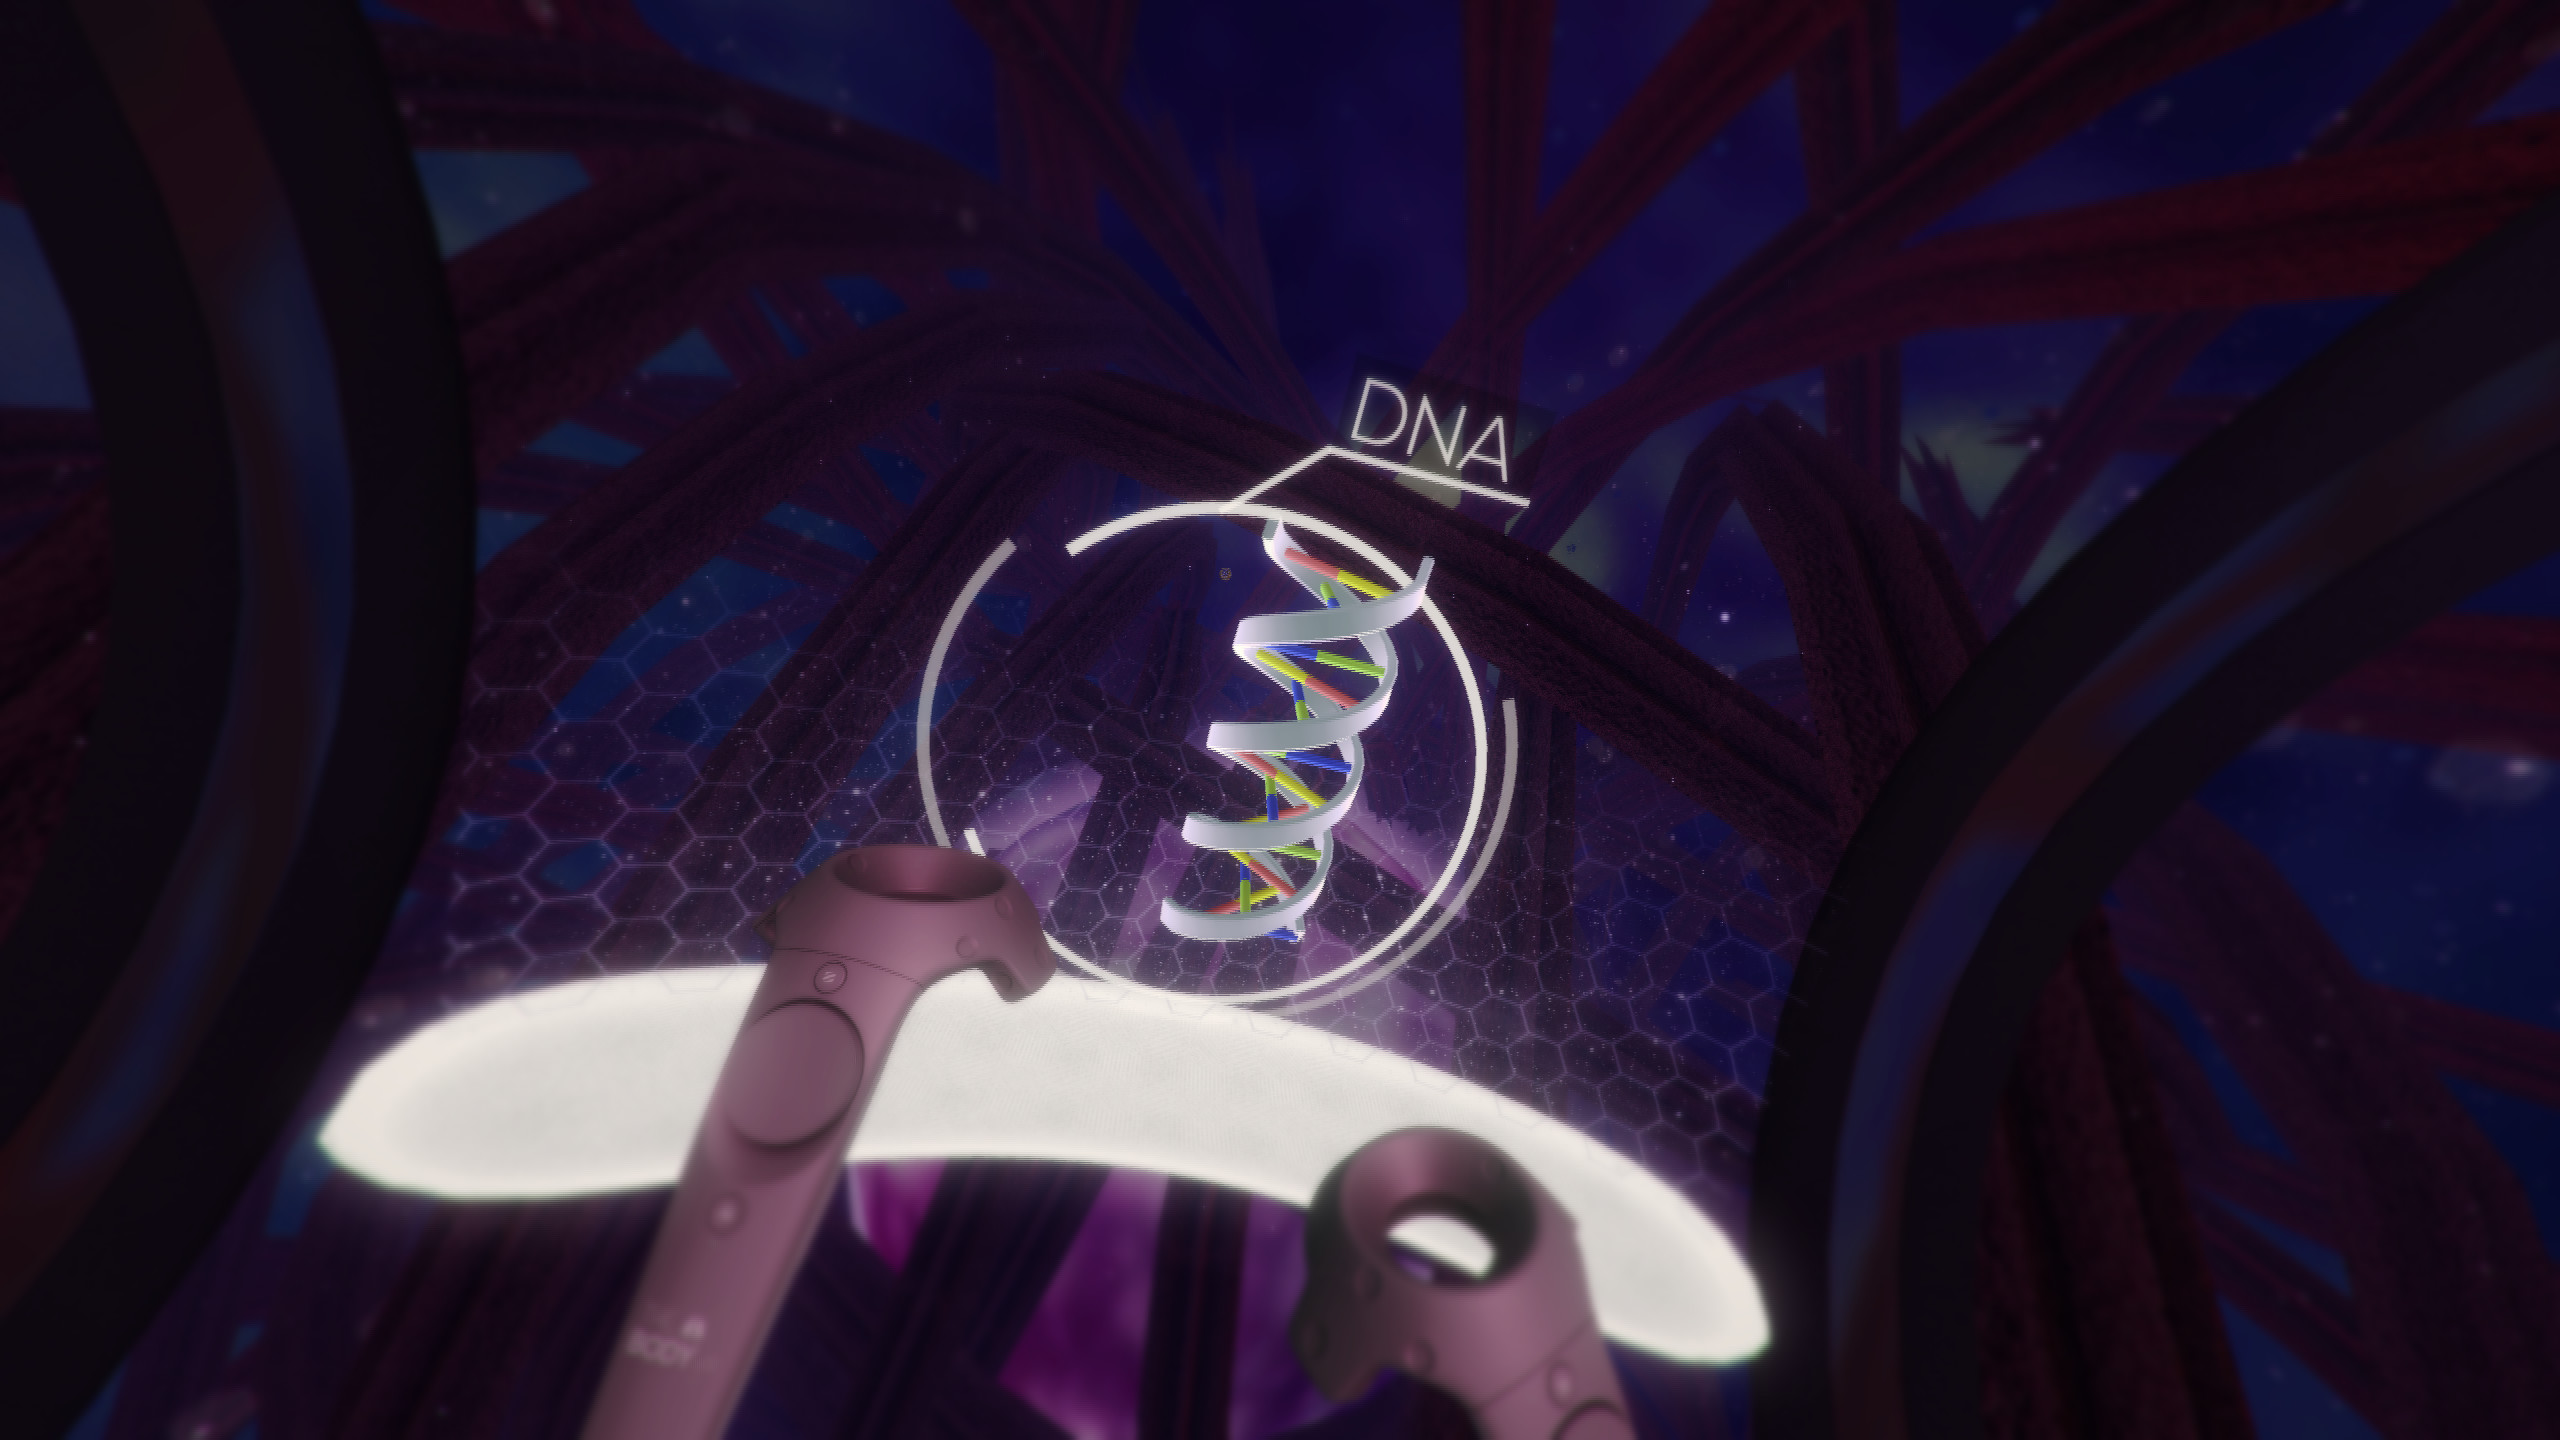
\includegraphics[width=0.65\textwidth]{bodyvr.jpg}
\caption{The~Body VR. \cite{the-body-vr-pic}}
\label{r:22}
\end{figure}

Most popular VR game nowadays is \textsl{Job Simulator}, an~experience for HTC Vive, taking place in a virtual world where robots have replaced all human jobs. Game's purpose is to teach, in a funny way, what it was like to have a job in the~past. It is the~most profitable VR experience on the~market, grossing more than \$3 million in sales. \cite{thesixthaxis.com}

\begin{figure}[ht!]
\centering
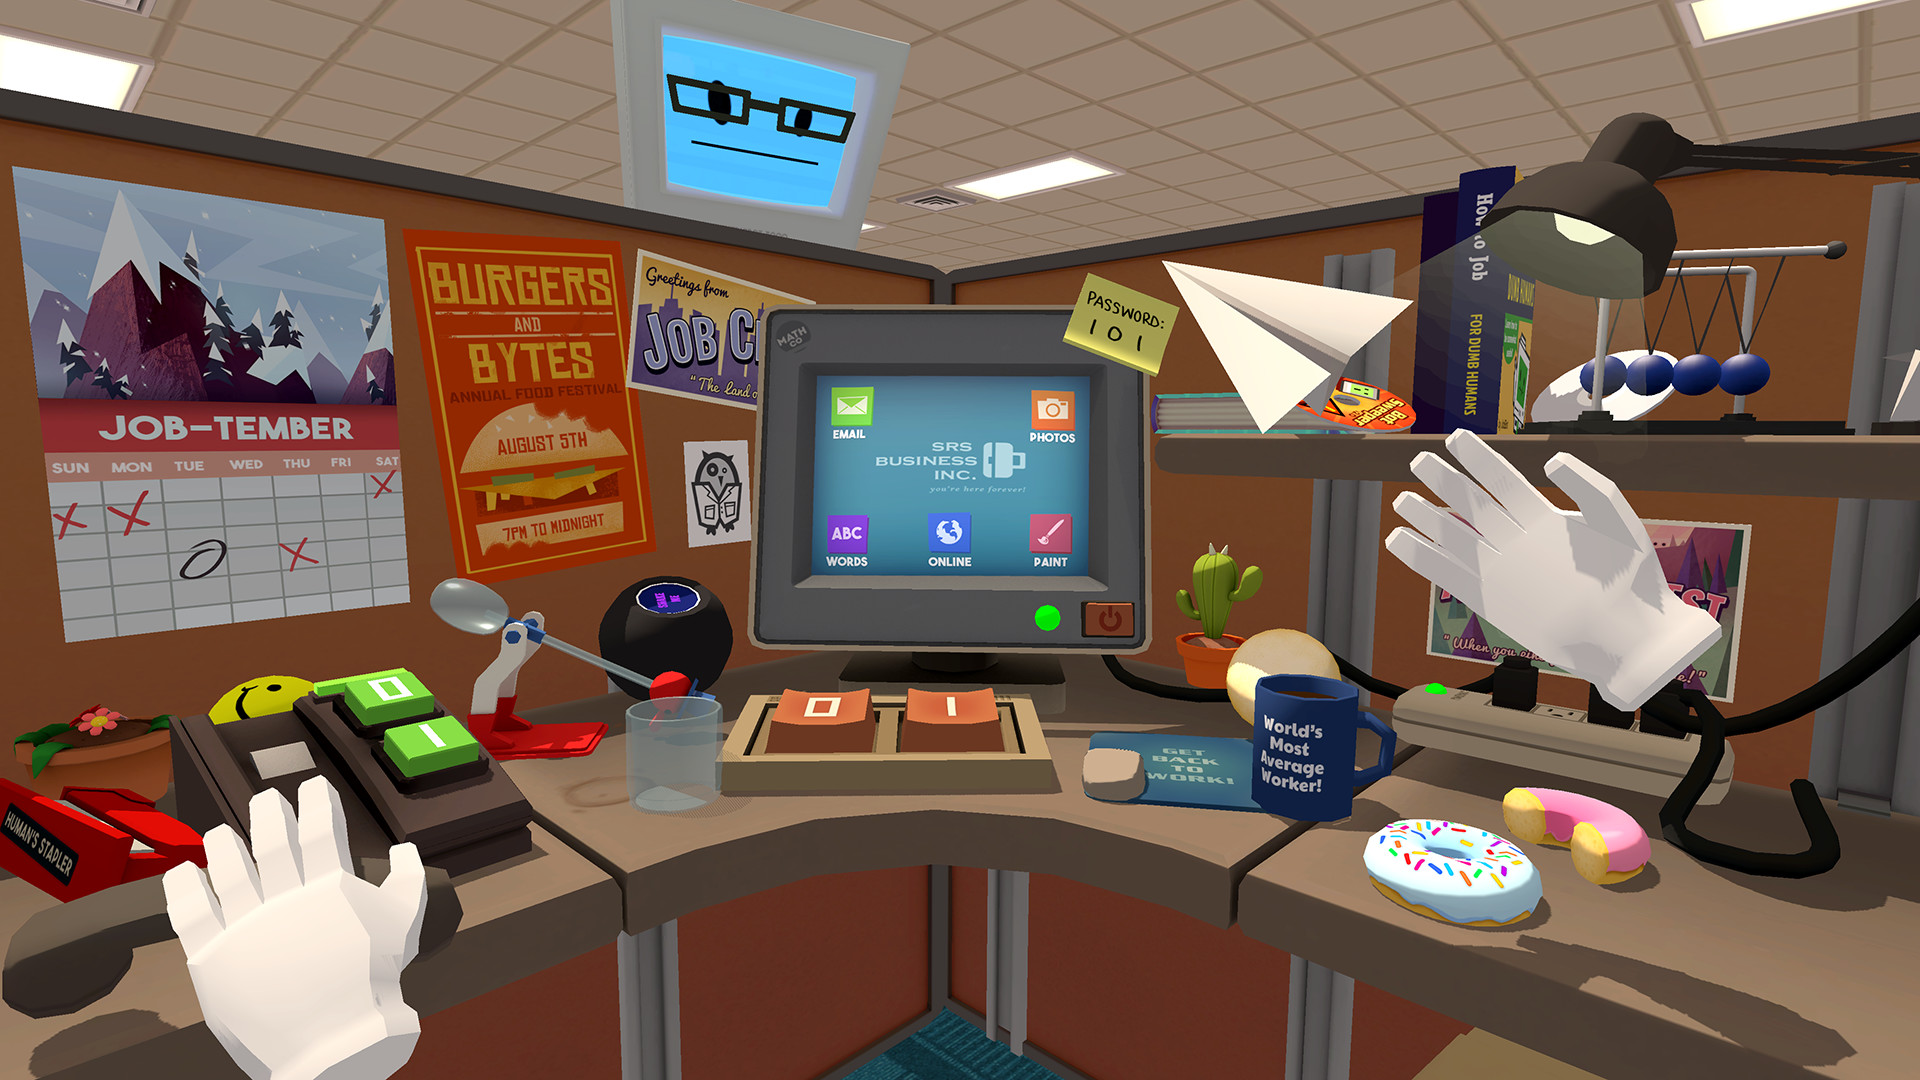
\includegraphics[width=0.65\textwidth]{job-simulator.jpg}
\caption{Job simulator. \cite{job-simulator-pic}}
\label{r:23}
\end{figure}

%\newpage
In field of mathematics, VR application named \textsl{Calcflow} is making serious progress. It's developed by \textsl{Nanome, Inc.} - a company that was started by students of \textsl{University of California San Diego} and stays affiliated with it. \textsl{Calcflow}'s features include visualizations of vector addition, cross product, parametrized functions, mobius strip, spherical coordinate mapping, double and surface integrals.

\begin{figure}[ht!]
\centering
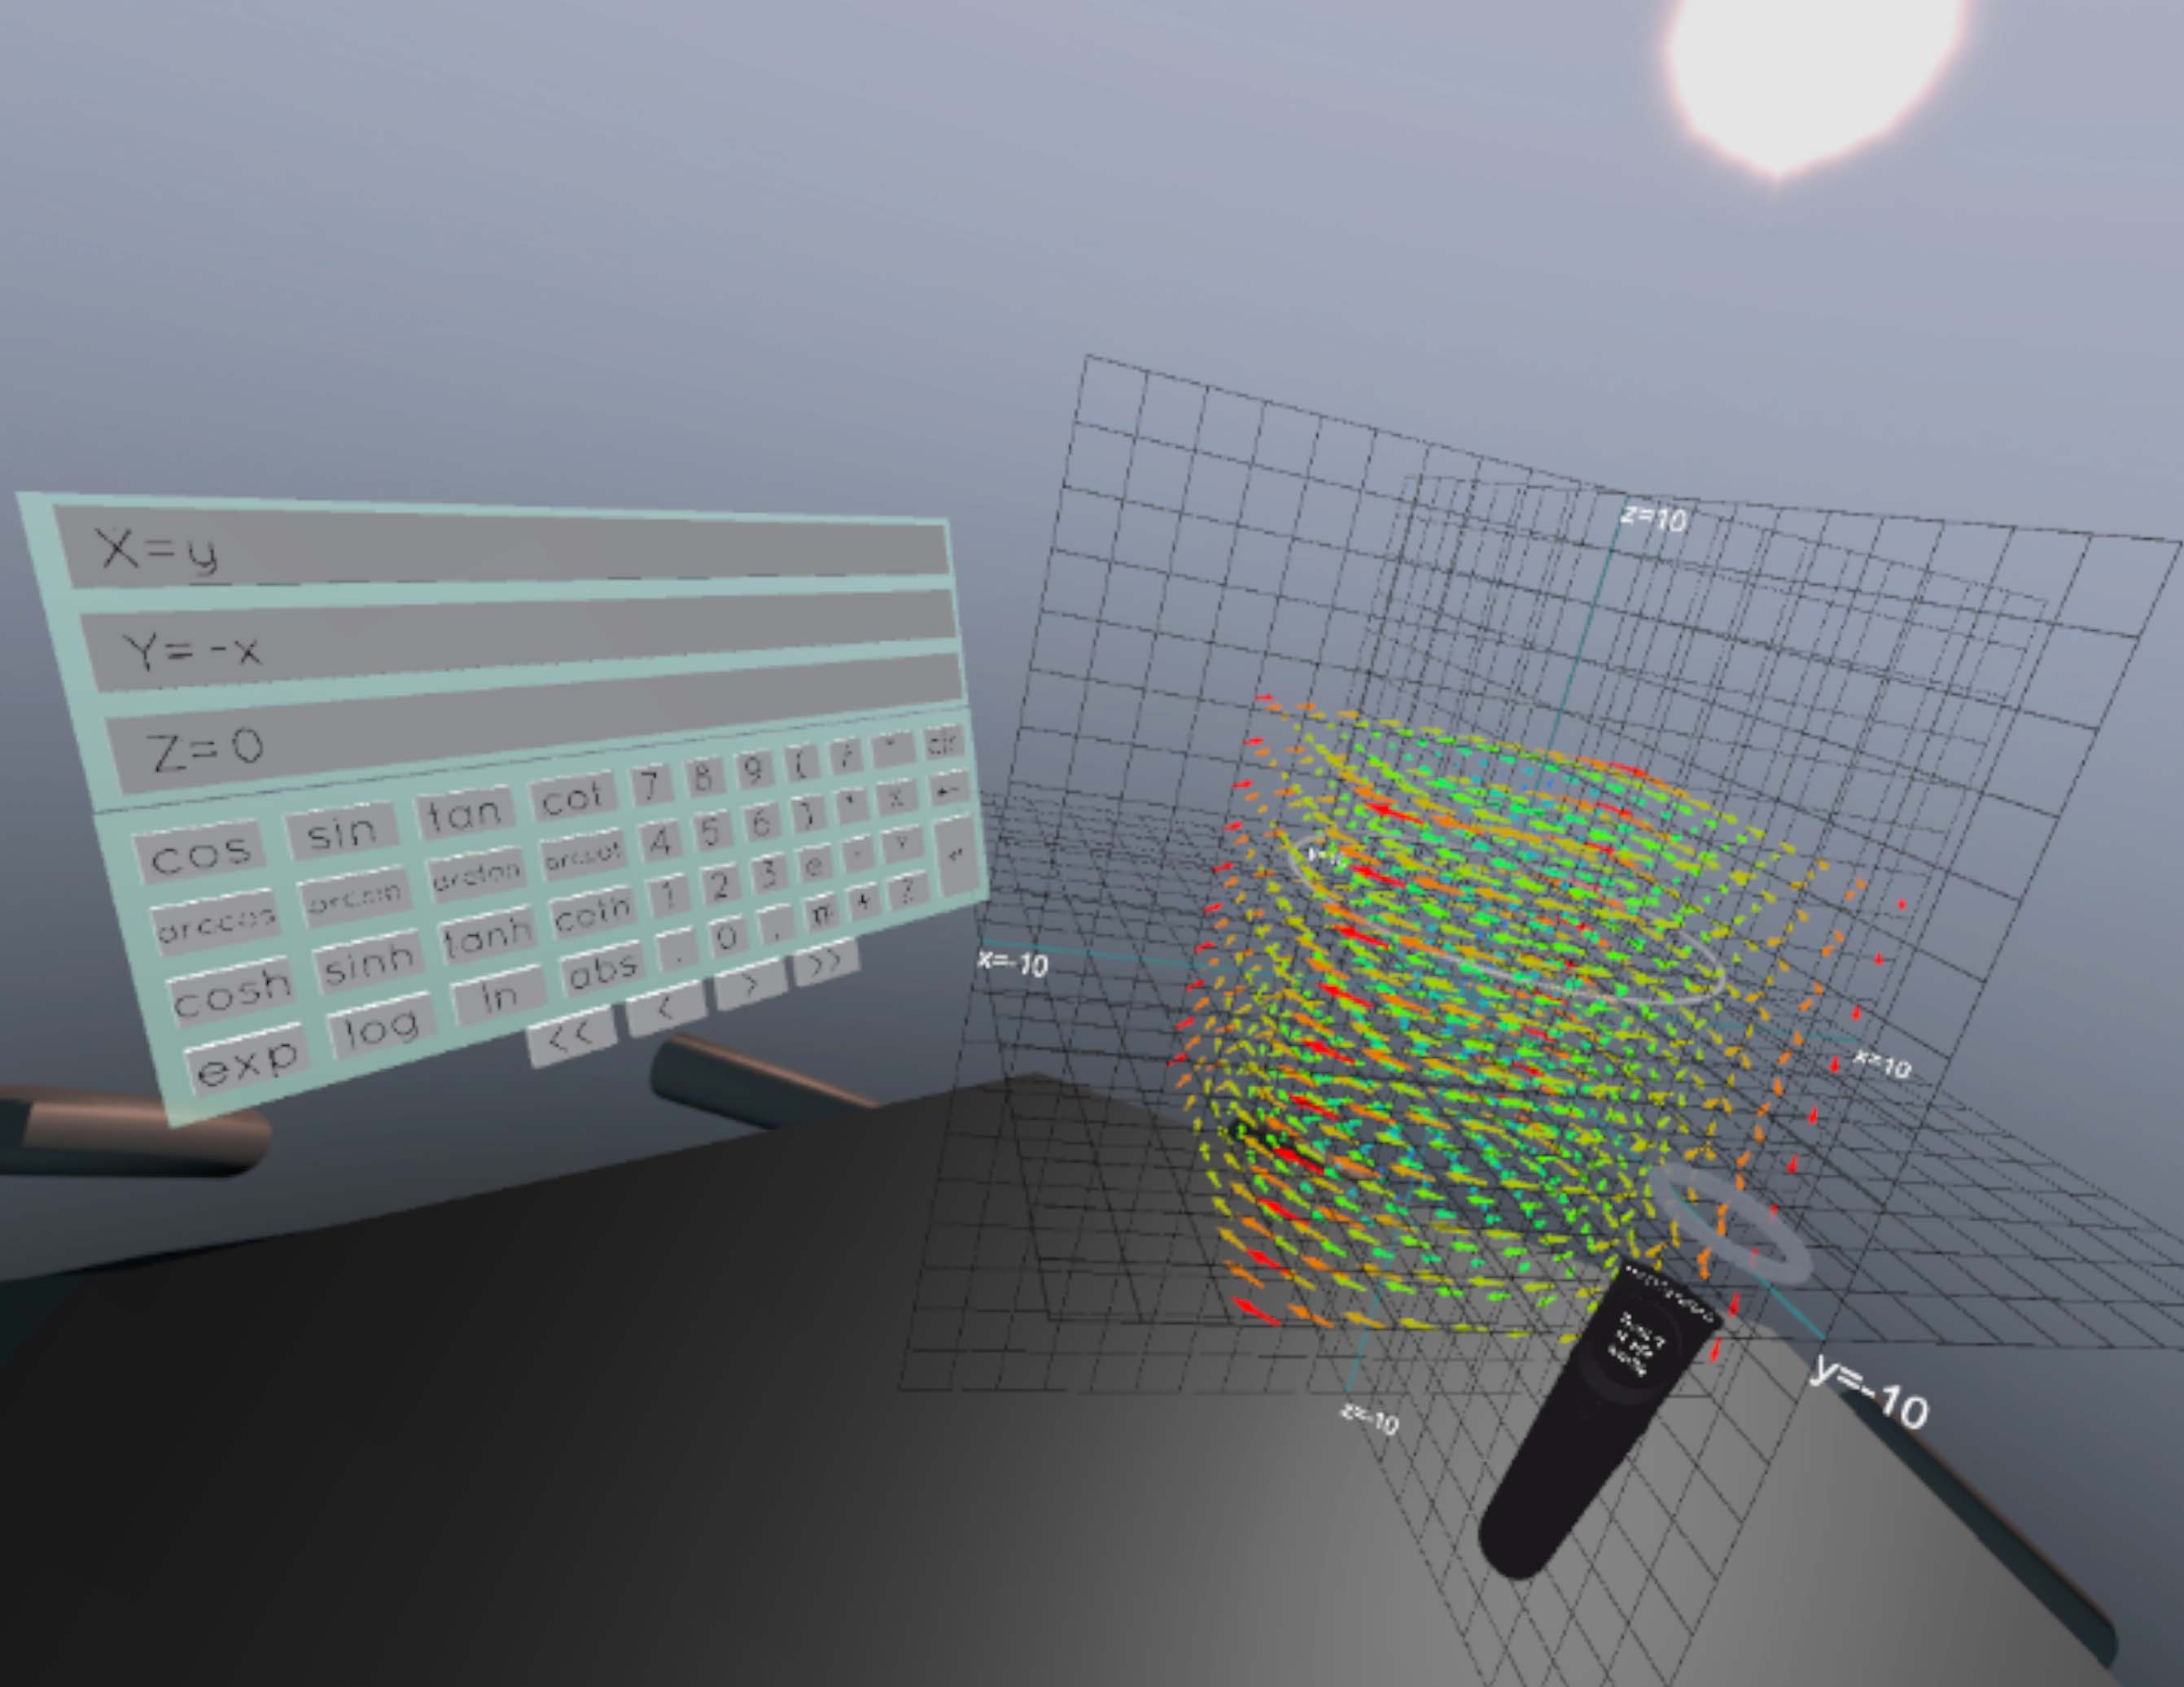
\includegraphics[width=0.8\textwidth]{calcflow.jpg}
\caption{Calcflow. \cite{calcflow-pic}}
\label{r:24}
\end{figure}

\subsection{Building virtual reality applications and experiences}
The~leading platform for building VR experiences today is the~game engine Unity, both because the~company had the~foresight to add support for the~Oculus Rift development kit early on, but also simply because the~early use cases from when Oculus Rift was still just a very successful Kickstarter project centered around video games.

Unreal Engine 4 is a complete suite of development tools made for anyone working with real-time technology. From enterprise applications and cinematic experiences to high-quality games across PC, console, mobile, VR and AR, Unreal Engine 4 gives developers everything they need to implement and deploy their games and experiences. \cite{unrealengine}

\subsection{Virtual reality on the~web}
WebVR provides support for exposing virtual reality devices — for example head-mounted displays like the~HTC Vive or Oculus Rift — to web apps, enabling developers to translate position and movement information from the~display into movement around a 3D scene in browser. As of today, support for both head-mounted displays is available in experimental or development builds of Chrome and Firefox, with official release planned for third quarter of 2017. This has numerous very interesting applications, from virtual product tours and interactive training apps to immersive first person games.
Unity game engine, for instance, is able to make native builds for all major platforms from the~same code base, including PC, Mac, Linux, iOS, Android and more. When made by professionals, such native builds will undoubtedly look better and run faster than a comparable VR experience built with WebGL and WebVR (at least AAA games or other experiences where high fidelity and performance are paramount).

The~major advantage of WebVR over natively built experiences is the~same as the~web has always had over desktop apps and mobile apps today - no need to download and install anything. User just needs to click a link, type in a url, and the~application runs directly in her browser. There’s no app store needed. Web developers can also take advantage of many open source libraries available on the~internet.

\section{Technologies and tools for development}
\subsection{JavaScript}
JavaScript is an~interpreted programming language with object-oriented (OO) capabilities. Syntactically, the~core JavaScript language resembles C, C++ and Java, with programming constructs such as the~if statement, the~while loop, and the~&& operator. Similarity ends with the~syntactic resemblance, however. JavaScript is a loosly typed language, which means that variables do not need to have a type specified. Object in JavaScript map property names to arbitrary property values. In this way they are more like hash tables or associative arrays (in Perl) then they are structs (in C) or objects (in C++ or Java). The~OO inheritance mechanism of JavaScript is prototype-based. This is different from inheritance in C++ and Java. \cite{flanagan}

JavaScript is mostly used in web browsers. It allows scripts to interact with the~user, control the~web browser and alter the~document content that appears within the~web browser window. This embedded version of JavaScript runs scripts embedded within HTML web pages. It's called client-side JavaScript to distinguish them from scripts that run on the~server, since JavaScript can also be used on server-side with Node.js. \cite{flanagan}

JavaScript programming language is standardized in the~ECMA-262 specification and ISO/IEC 16262 by standards organization European Computer Manufacturers Association (ECMA) and is often refered to as ECMAScript. Most popular browsers currently supports ECMAScript in version 5 (ES5). ECMAScript 6 (ES6) is the~sixth version seventh edition of ECMAScript language which was introduced to improve JavaScript and ensure that developers no longer needed to use abstractions or other techniques to write quality code.\cite{narayan}

\subsection{NPM}
NPM is the~package manager for JavaScript and the~world’s largest software registry, which makes it easy for JavaScript developers to share the~code that they've created to solve particular problems, and for other developers to reuse that code in their own applications.\cite{npm}

The~bits of reusable code are called packages, or sometimes modules. A package is just a directory with one or more files in it, that also has a file called "package.json" with some metadata about this package. A typical application, such as a website, will depend on dozens or hundreds of packages. These packages are often small. The~general idea is to create a small building block which solves one problem and solves it well. This makes it possible for developers to compose larger, custom solutions out of these small, shared building blocks.\cite{npm}

There's lots of benefits to this. It makes it possible for development teams to draw on expertise outside of the~organization they are working in by bringing in packages from people who have focused on particular problem areas. But even if they don't reuse code from people outside of the~organization, using this kind of module based approach can actually help the~team work together better, and can also make it possible to reuse code across projects.\cite{npm}

We can find packages to help us build our application by browsing the~npm website. When we're browsing the~website, we'll find different kinds of packages and node modules. NPM started as the~node package manager, so we'll find lots of modules which can be used on the~server side. There are also packages which add commands for us to use in the~command line.\cite{npm} And there are a number of packages which can be used in the~browser, on the~front end, which we're going to use in our project, MathworldVR.

\subsection{Three.js}
Three.js is cross-browser JavaScript library/API used to create and display animated 3D computer graphics in a web browser. It uses WebGL.

\subsection{A-Frame}
A-Frame is a web framework for building virtual reality experiences. It was started by Mozilla to make WebVR content creation easier, faster, and more accessible. A-Frame lets you build scenes with just HTML while having unlimited access to JavaScript, Three.js, and all existing Web APIs. It uses an~entity-component-system pattern that promotes composition and extensibility. It is free and open source with growing community and a ecosystem of tools and components. \cite{aframe-intro}

There are no build steps or boilerplate required to install, we just need an~HTML file:

\begin{lstlisting}
<html>
  <head>
    <script src="https://aframe.io/releases/0.5.0/aframe.min.js"></script>
  </head>
  <body>
    <a-scene>
      <a-box color="#6173F4" opacity="0.8" depth="2"></a-box>
      <a-sphere radius="2" src="texture.png" position="1 1 0"></a-sphere>
      <a-sky color="#ECECEC"></a-sky>
    </a-scene>
  </body>
</html>
\end{lstlisting}

\texttt{<a-scene>} contains all of the~objects in 3D scene. It also handles all of the~setup that is traditionally required for 3D: setting up WebGL, the~canvas, camera, lights, renderer, render loop as well as out of the~box VR support on platforms such as HTC Vive, Oculus Rift, Samsung GearVR, and smartphones (Google Cardboard). We can place objects within our scene using assorted primitive elements that come with A-Frame such as \texttt{<a-box>} or \texttt{<a-sphere>}. This approach helps with keeping the~codebase readable. We could copy and paste this HTML to any other scene and it would behave in the~same way. \cite{aframe-intro}

\subsubsection{JavaScript and Aframe}
We can use traditional JavaScript DOM APIs to manipulate A-Frame scenes to add logic, behavior, and functionality:

\begin{lstlisting}
var box = document.querySelector('a-box');
box.getAttribute('position');
box.addEventListener('click', function () {
  box.setAttribute('color', 'red');
});
\end{lstlisting}

A-Frame components are being based on the~DOM, so most existing client-side libraries and frameworks such as React, Vue.js, d3.js, jQuery, or Angular work on top of A-Frame. The~existing web ecosystem of tools were built on top of the~notion of manipulating plain HTML and are thus compatible with A-Frame. \cite{aframe-intro}

\subsubsection{Entity-Component System}
A-Frame at its core is an~entity-component-system framework. Entity-component-system (ECS) is a pattern popular in game development and is prominent in game engines like Unity. ECS favors composition over inheritance. Every single object in the~scene is an~entity. an~entity is an~empty placeholder object that by itself does nothing. We plug in reusable components to attach appearance, behavior or functionality. We can also put different components together and configure them in order to define different types of objects. \cite{aframe-intro}

Object-oriented and hierarchical patterns have well-suited the~2D web, where we lay out elements and components that have fixed behavior on a web page. 3D and VR is different; there are infinite types of objects with endless complexity. A-Frame provides an~easy way to build up different kinds of objects without having to create a special class for each one. \cite{aframe-intro}

In A-Frame, an~entity is simply an~HTML tag:

\begin{lstlisting}
<a-entity></a-entity>
\end{lstlisting}

A-Frame components are reusable modules that can be plugged into any entity. They are allowed to do anything and have full access to JavaScript, Three.js, and Web APIs. The~structure of a basic component may look like this:

\begin{lstlisting}
AFRAME.registerComponent('foo', {
  schema: {
    bar: {type: 'number'},
    baz: {type: 'string'}
  },
  init: function () {
    // Do something when component is plugged in.
  },
  update: function () {
    // Do something when component's data is updated.
  }
});
\end{lstlisting}

\newpage
Then once defined, we can plug this bundle of appearance, behavior, or functionality into an~entity straight from an~HTML attribute:

\begin{lstlisting}
<a-entity foo="bar: 5; baz: qux"></a-entity>
\end{lstlisting}

\subsubsection{Component Ecosystem}
A-Frame ships with several components, but since A-Frame is fully extensible at its core, the~community provided the~ecosystem with lot's of components such as physics, particle systems, audio visualizations, and Leap Motion controls. This ecosystem is the~driving force behind the~popularization of A-Frame. Developer can build a component, publish it, and then someone else can take that component and use it straight from HTML without having to know JavaScript. \cite{aframe-intro}

These components are curated and collected into the~A-Frame Registry. This is similar to the~collection of components and modules on the~Unity Asset Store or NPM, but free and open source. A-Frame maintainers and core developers make sure they work well and from there they are easily searchable and installable through multiple channels, one of which is through the~A-Frame Inspector. \cite{aframe-intro}

\subsubsection{A-Frame Inspector}
The~A-Frame Inspector is a visual tool for inspecting and editing A-Frame scenes. Similar to the~browser’s DOM Inspector, you can go to any A-Frame scene, local or on the~Web, and hit \texttt{<ctrl>} + \texttt{<alt>} + \texttt{i} on your keyboard. This will open the~visual Inspector where you can make changes and return to the~scene with the~reflected changes. You can visually move and place objects, change properties of the~components, or pan the~camera around to see a different view of the~scene. It’s similar to viewing the~source code in an~interactive way. The~A-Frame Inspector is integrated with the~A-Frame Registry. From the~Inspector, you can install components from the~Registry and attach them to objects in the~scene. \cite{aframe-intro}

\begin{figure}[ht!]
\centering
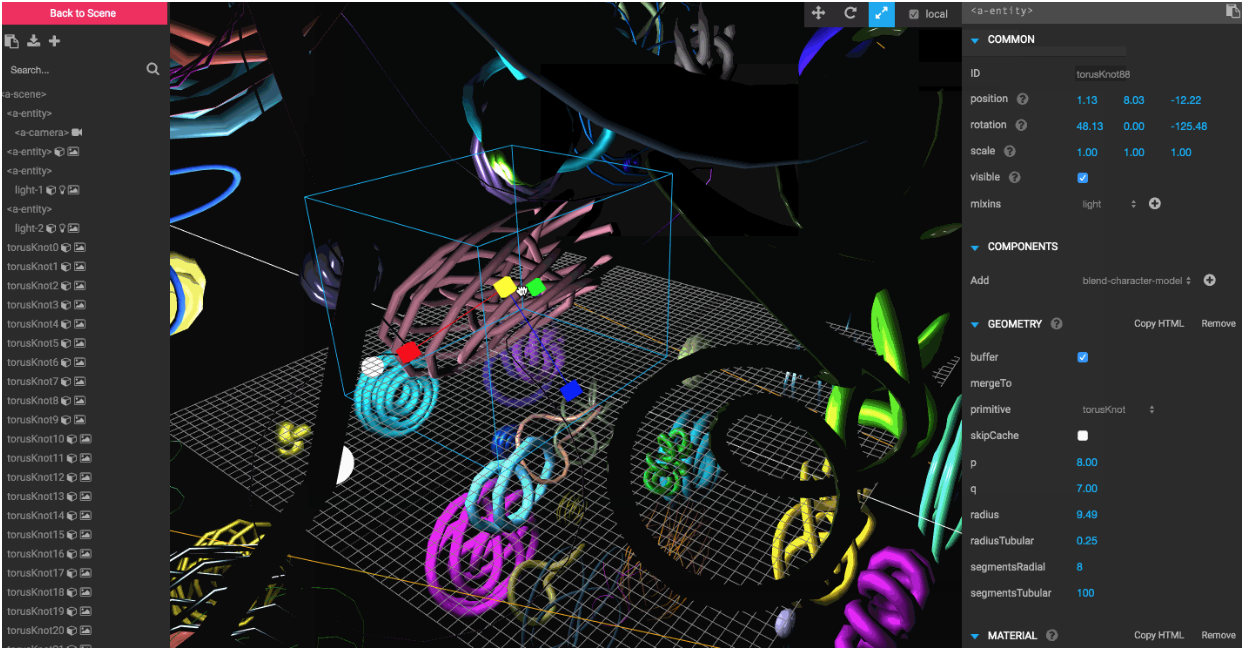
\includegraphics[width=0.9\textwidth]{aframe-inspector}
\caption{A-Frame Inspector window.}
\label{r:41}
\end{figure}

\subsubsection{Device and Platform Support}
Devices and platform support depends on how well the~browsers support certain devices and APIs. A-Frame supports both flat (3D on a normal screen) and WebVR experiences, though its focus is heavily VR. Support for flat experiences primarily depends on a browser’s WebGL support. We can see which browsers support WebGL at \url{http://caniuse.com/#feat=webgl}. Support for VR experiences, along with WebGL support, depends on a browser’s support for the~WebVR API. You can see which browsers currently support the~WebVR API at \url{https://webvr.rocks}. A-Frame supports version 1.0 of the~WebVR API. The~exception to this is for mobile devices, which are supported through the~WebVR Polyfill. A-Frame currently supports controllers with six degrees of freedom (6DoF) using experimental build of Chromium browser with experimental controller support (e.g., Vive controllers). \cite{aframe-intro}

\subsection{Math.js}
\textsl{Math.js is an~extensive math library for JavaScript and Node.js. It features a flexible expression parser with support for symbolic computation, comes with a large set of built-in functions and constants, and offers an~integrated solution to work with different data types like numbers, big numbers, complex numbers, fractions, units, and matrices.} \cite{mathjs}

\subsection{React}
ReactJS is a javascript library for building user interfaces, originally created by engineers at Facebook to solve the~challenges involved when developing complex user interfaces with datasets that change over time. It provides a way to write encapsulated components that manage their own state, then compose them to make complex user interfaces. It doesn't make assumptions about the~rest of the~technology stack, because it’s just library. Since component logic is written in JavaScript instead of templates, we can easily pass rich data through our app and keep state out of the~DOM. \cite{gackenheimer}

\subsection{Flux}
Flux is an~application architecture created by Facebook for building client-side web applications. It complements the~React in a way that displaces the~standard Model-View-Controller (MVC) framework. It was designed in React in mind and aims to help developers to create more efficient, maintainable code when dissecting the~application into multiple components, which according to Facebook engineers was hard if the~traditional MVC pattern was followed when building the~application with React.\citep{gackenheimer}

\textsl{Flux is utilizing a unidirectional data flow. It's more of a pattern rather than a formal framework, and developers can start using Flux immediately without a lot of new code.} \citep{flux}

\textsl{Flux applications have three major parts: the~dispatcher, the~stores, and the~views (React components). These should not be confused with Model-View-Controller. Controllers do exist in a Flux application, but they are controller-views - views often found at the~top of the~hierarchy that retrieve data from the~stores and pass this data down to their children. Additionally, action creators - dispatcher helper methods - are used to support a semantic API that describes all changes that are possible in the~application.} \citep{flux}

\textsl{Flux abandons MVC in favor of a uni-directional data flow. When a user interacts with a React view, the~view propagates an~action through a central dispatcher, to the~various stores that hold the~application's data and business logic, which updates all of the~views that are affected. This works especially well with React's declarative programming style, which allows the~store to send updates without specifying how to transition views between states.} \citep{flux}

\subsubsection{Structure and Data Flow in Flux architecture}
\textsl{A uni-directional data flow is the~main consequence of using the~Flux pattern, and the~diagram below should be the~primary mental model for the~Flux programmer. The~dispatcher, stores and views are independent nodes with distinct inputs and outputs. The~actions are simple objects containing a action type that identifies the~property and the~new data that is passed along with the~action.} \citep{flux}

\begin{figure}[ht!]
\centering
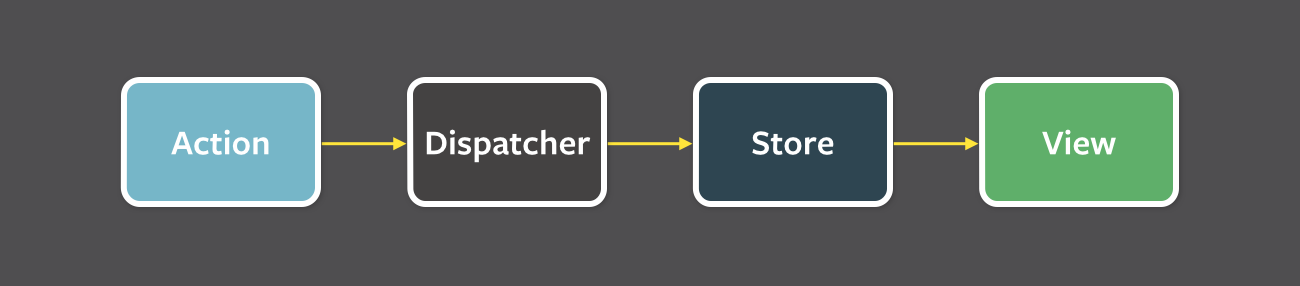
\includegraphics[width=1\textwidth]{flux-simple-f8-diagram}
\caption{Data in a Flux application flows in a single direction. \citep{flux}}
\label{r:42}
\end{figure}

\textsl{The~views may cause a new action to be propagated through the~system in response to user interactions.} \citep{flux}

\textsl{All data flows through the~dispatcher as a central hub. Actions are provided to the~dispatcher in an~action creator method, and most often originate from user interactions with the~views. The~dispatcher then invokes the~callbacks that the~stores have registered with it, dispatching actions to all stores. Within their registered callbacks, stores respond to whichever actions are relevant to the~state they maintain. The~stores then emit a change event to alert the~controller-views that a change to the~data layer has occurred. Controller-views listen for these events and retrieve data from the~stores in an~event handler. The~controller-views call their own setState() method, causing a re-rendering of themselves and all of their descendants in the~component tree.} \citep{flux}

\begin{figure}[ht!]
\centering
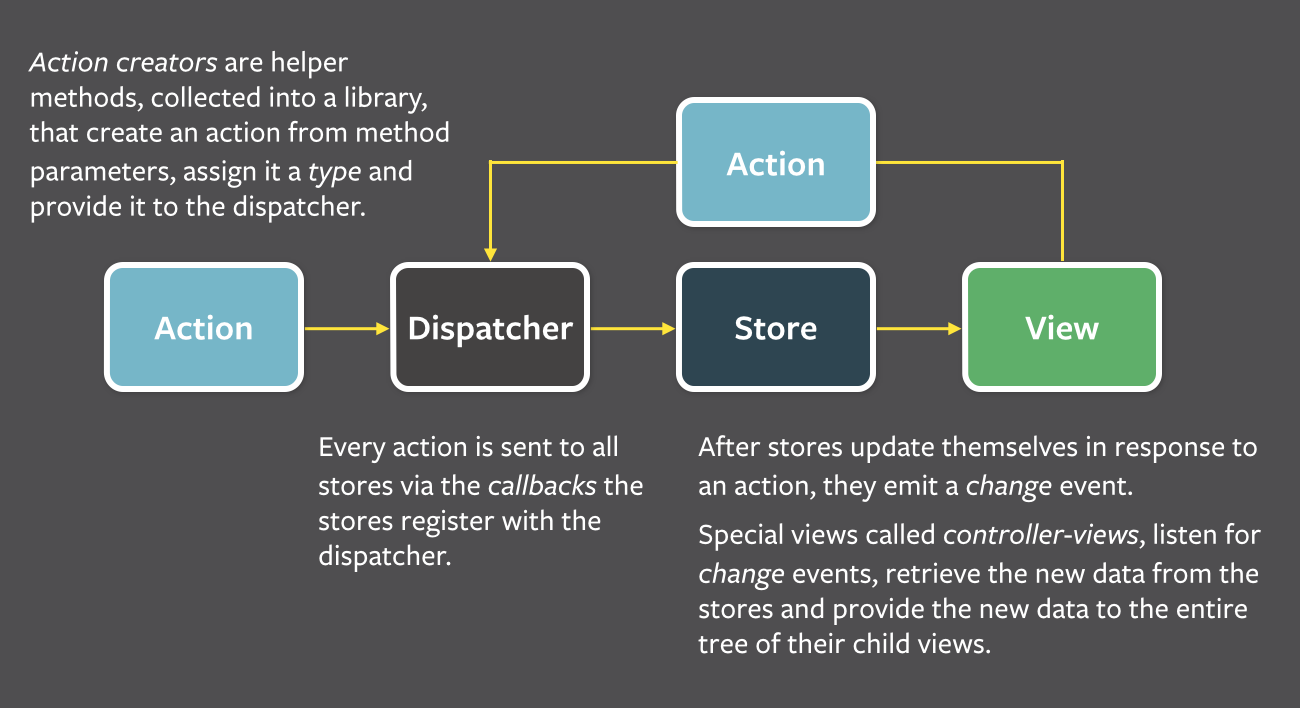
\includegraphics[width=0.9\textwidth]{flux-simple-f8-diagram-explained}
\caption{Detailed Flux application architecture diagram. \citep{flux}}
\label{r:43}
\end{figure}

\textsl{This structure allows us to reason easily about our application in a way that is reminiscent of functional reactive programming, or more specifically data-flow programming or flow-based programming, where data flows through the~application in a single direction — there are no two-way bindings. Application state is maintained only in the~stores, allowing the~different parts of the~application to remain highly decoupled.} \citep{flux}

\textsl{We found that two-way data bindings led to cascading updates, where changing one object led to another object changing, which could also trigger more updates. As applications grew, these cascading updates made it very difficult to predict what would change as the~result of one user interaction. When updates can only change data within a single round, the~system as a whole becomes more predictable.} \citep{flux}

\subsection{Redux}
Redux is a predictable state container for JavaScript applications, inspired by several important qualities of Flux architecture. It helps developers write applications that behave consistently, run in different environments (client, server, and native), and are easy to test. On top of that, it provides a great developer experience, such as live code editing combined with a time traveling debugger.\citep{redux-intro} We are using Redux together with React, but in general it can be used with any other view library.

The~whole state of application is stored in an~object tree inside a single store. The~only way to change the~state tree is to emit an~action, an~object describing what happened. To specify how the~actions transform the~state tree, we write pure reducers.\citep{redux-intro}

Instead of mutating the~state directly, we specify the~mutations we want to happen with plain objects called actions. Then we write a special function called a reducer to decide how every action transforms the~entire application's state.\citep{redux-intro}

Unlike Flux, Redux does not have the~concept of a Dispatcher. This is because it relies on pure functions instead of event emitters, and pure functions are easy to compose and don't need an~additional entity managing them.

The~beauty and strength of this pattern is how well it scales to large and complex apps. It also enables very powerful developer tools, because it is possible to trace every mutation to the~action that caused it. We can record user sessions and reproduce them just by replaying every action.\citep{redux-intro}

\subsubsection{Three Principles of Redux}
\textbf{1. Single source of truth}

\textsl{The~state of your whole application is stored in an~object tree within a single store. This makes it easy to create universal apps, as the~state from your server can be serialized and hydrated into the~client with no extra coding effort. A single state tree also makes it easier to debug or inspect an~application; it also enables you to persist your app's state in development, for a faster development cycle. Some functionality which has been traditionally difficult to implement - Undo/Redo, for example - can suddenly become trivial to implement, if all of your state is stored in a single tree.} \citep{redux-intro}

\textbf{2. State is read-only}

\textsl{The~only way to change the~state is to emit an~action, an~object describing what happened. This ensures that neither the~views nor the~network callbacks will ever write directly to the~state. Instead, they express an~intent to transform the~state. Because all changes are centralized and happen one by one in a strict order, there are no subtle race conditions to watch out for. As actions are just plain objects, they can be logged, serialized, stored, and later replayed for debugging or testing purposes.} \citep{redux-intro}

\textbf{3. Changes are made with pure functions}

\textsl{To specify how the~state tree is transformed by actions, you write pure reducers. Reducers are just pure functions that take the~previous state and an~action, and return the~next state. Remember to return new state objects, instead of mutating the~previous state. You can start with a~single reducer, and as your app grows, split it off into smaller reducers that manage specific parts of the~state tree. Because reducers are just functions, you can control the~order in which they are called, pass additional data, or even make reusable reducers for common tasks such as pagination.} \citep{redux-intro}

\subsection{Webpack}
Webpack is a~module bundler for modern JavaScript applications. It takes modules with dependencies and generates static assets representing those modules [\ref{r:45}]. Its strength is that it's configurable and developers using it in their applications should know the~four core concepts used when configuring Webpack:

\begin{itemize}
\item Entry - Webpack creates a~graph of all of your application's dependencies and the~starting point of this graph is called entry point. It tells Webpack where to start and follows the~graph of dependencies to know what to bundle.
\item Output - it tells Webpack where to bundle our application.
\item Loaders - Webpack treats every file (.css, .html, .scss, .jpg, etc.) as a~module. However, webpack only understands JavaScript, so loaders transform these files into modules as they are added to dependency graph.
\item Plugins - loaders only execute transform on per-file basis, but plugins are mostly used to perform actions and custom functionality on combilations or chunks of bundled modules.
\end{itemize}

\begin{figure}[ht!]
\centering
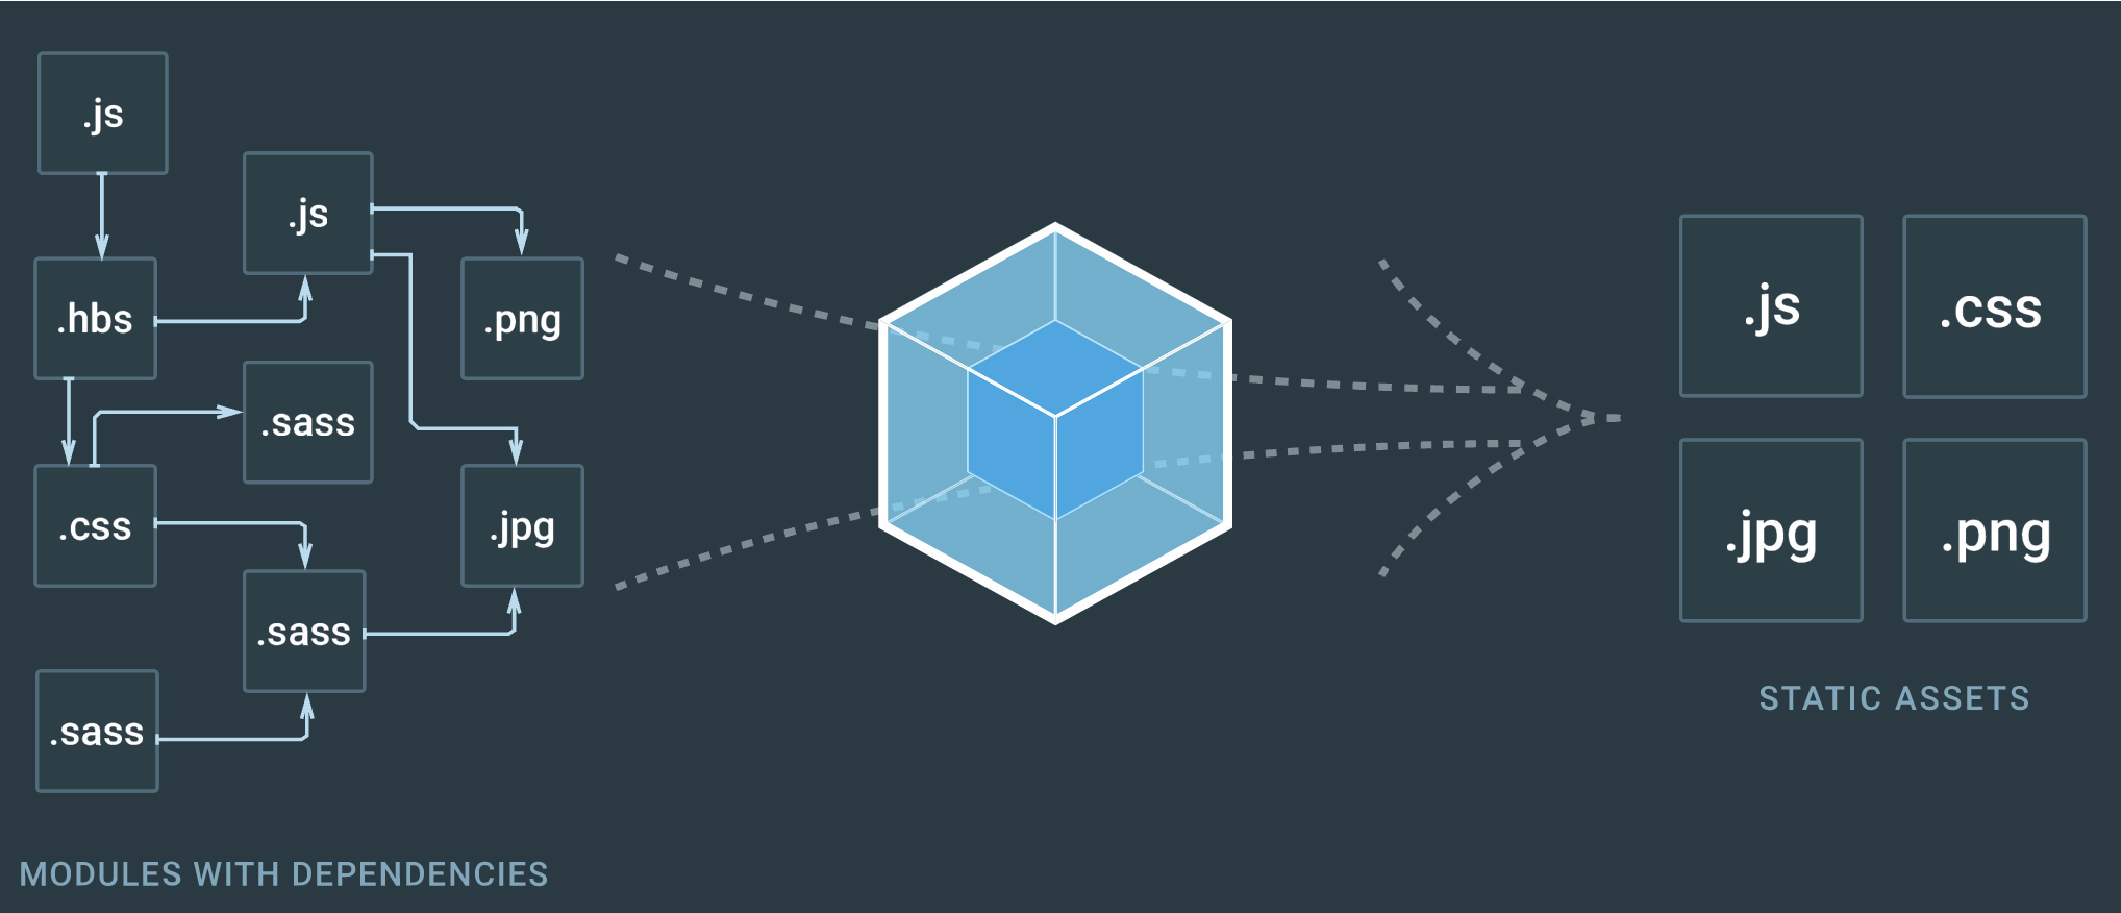
\includegraphics[width=0.9\textwidth]{webpack}
\caption{Bundling dependencies and static assets with Webpack}
\label{r:45}
\end{figure}